\documentclass{scrbook}

%!TEX root = thesis.tex

% Set german to default language and load english as well
\usepackage[english,ngerman]{babel}

% Set UTF8 as input encoding
\usepackage[utf8]{inputenc}

% Set T1 as font encoding
\usepackage[T1]{fontenc}
% Load a slightly more modern font
\usepackage{lmodern}
% Use the symbol collection textcomp, which is needed by listings.
\usepackage{textcomp}
% Load a better font for monospace.
\usepackage{courier}

% Set some options regarding the document layout. See KOMA guide
\KOMAoptions{%
  paper=a4,
  fontsize=12pt,
  parskip=half,
  headings=normal,
  BCOR=1cm,
  headsepline,
  DIV=12}

% do not align bottom of pages
\raggedbottom

% set style of captions
\setcapindent{0pt} % do not indent second line of captions
\setkomafont{caption}{\small}
\setkomafont{captionlabel}{\bfseries}
\setcapwidth[c]{0.9\textwidth}

% set the style of the bibliography
\bibliographystyle{alphadin}

% load extended tabulars used in the list of abbreviation
\usepackage{tabularx}

% load the color package and enable colored tables
\usepackage[table]{xcolor}

% define new environment for zebra tables
\newcommand{\mainrowcolors}{\rowcolors{1}{maincolor!25}{maincolor!5}}
\newenvironment{zebratabular}{\mainrowcolors\begin{tabular}}{\end{tabular}}
\newcommand{\setrownumber}[1]{\global\rownum#1\relax}
\newcommand{\headerrow}{\rowcolor{maincolor!50}\setrownumber1}

% add main color to section headers
\addtokomafont{chapter}{\color{maincolor}}
\addtokomafont{section}{\color{maincolor}}
\addtokomafont{subsection}{\color{maincolor}}
\addtokomafont{subsubsection}{\color{maincolor}}
\addtokomafont{paragraph}{\color{maincolor}}

% do not print numbers next to each formula
\usepackage{mathtools}
\mathtoolsset{showonlyrefs}
% left align formulas
\makeatletter
\@fleqntrue\let\mathindent\@mathmargin \@mathmargin=\leftmargini
\makeatother

% Allow page breaks in align environments
\allowdisplaybreaks

% header and footer
\usepackage{scrpage2}
\pagestyle{scrheadings}
\setkomafont{pagenumber}{\normalfont\sffamily\color{maincolor}}
\setkomafont{pageheadfoot}{\normalfont\sffamily}
\setheadsepline{0.5pt}[\color{maincolor}]

% German guillemets quotes
\usepackage[german=guillemets]{csquotes}

% load TikZ to draw diagrams
\usepackage{tikz}

% load additional libraries for TikZ
\usetikzlibrary{%
  automata,%
  positioning,%
}

% set some default options for TikZ -- in this case for automata
\tikzset{
  every state/.style={
    draw=maincolor,
    thick,
    fill=maincolor!18,
    minimum size=0pt
  }
}

% load listings package to typeset sourcecode
\usepackage{listings}

% set some options for the listings package
\lstset{%
  upquote=true,%
  showstringspaces=false,%
  basicstyle=\ttfamily,%
  keywordstyle=\color{keywordcolor}\slshape,%
  commentstyle=\color{commentcolor}\itshape,%
  stringstyle=\color{stringcolor}}

% enable german umlauts in listings
\lstset{
  literate={ö}{{\"o}}1
           {Ö}{{\"O}}1
           {ä}{{\"a}}1
           {Ä}{{\"A}}1
           {ü}{{\"u}}1
           {Ü}{{\"U}}1
           {ß}{{\ss}}1
}

% define style for pseudo code
\lstdefinestyle{pseudo}{language={},%
  basicstyle=\normalfont,%
  morecomment=[l]{//},%
  morekeywords={for,to,while,do,if,then,else},%
  mathescape=true,%
  columns=fullflexible}

% load the AMS math library to typeset formulas
\usepackage{amsmath}
\usepackage{amsthm}
\usepackage{thmtools}
\usepackage{amssymb}

% load the paralist library to use compactitem and compactenum environment
\usepackage{paralist}

% load varioref and hyperref to create nicer references using vref
\usepackage[ngerman]{varioref}
\PassOptionsToPackage{hyphens}{url} % allow line break at hyphens in URLs
\usepackage{hyperref}

% setup hyperref
\hypersetup{breaklinks=true,
            pdfborder={0 0 0},
            ngerman,
            pdfhighlight={/N},
            pdfdisplaydoctitle=true}

% Fix bugs in some package, e.g. listings and hyperref
\usepackage{scrhack}

% define german names for referenced elements
% (vref automatically inserts these names in front of the references)
\labelformat{figure}{Abbildung\ #1}
\labelformat{table}{Tabelle\ #1}
\labelformat{appendix}{Anhang\ #1}
\labelformat{chapter}{Kapitel\ #1}
\labelformat{section}{Abschnitt\ #1}
\labelformat{subsection}{Unterabschnitt\ #1}
\labelformat{subsubsection}{Unterunterabschnitt\ #1}

% define theorem environments
\declaretheorem[numberwithin=chapter,style=plain]{Theorem}
\labelformat{Theorem}{Theorem\ #1}

\declaretheorem[sibling=Theorem,style=plain]{Lemma}
\labelformat{Lemma}{Lemma\ #1}

\declaretheorem[sibling=Theorem,style=plain]{Korollar}
\labelformat{Korollar}{Korollar\ #1}

\declaretheorem[sibling=Theorem,style=definition]{Definition}
\labelformat{Definition}{Definition\ #1}

\declaretheorem[sibling=Theorem,style=definition]{Beispiel}
\labelformat{Beispiel}{Beispiel\ #1}

\declaretheorem[sibling=Theorem,style=definition]{Bemerkung}
\labelformat{Bemerkung}{Bemerkung\ #1}

%!TEX root = thesis.tex

% Use this file to define some macros you need in your thesis. A macro is a short command that inserts some mathematical symbols or texts you do not want to retype each time you need some. I recommend to use as many macros as possible, because you are able to change them later. For example if you use the same macro each time you need to give the formal semantics of an expression you can easily change the appearance of these brackets by updating the macro later on.

% Set of natural numbers
\newcommand{\N}{\mathbb{N}}

% The default epsilon does not look very nice
\let\epsilon\varepsilon

% If you need to use mathematical expressins like an epsilon in the section titles of your thesis you will end up with warnings that these special symbols cannot be included in the PDF favorites. The following macro uses the mathematical symbol during the text of the thesis and the string "Epsilon" in the PDF favorites.
\newcommand{\pdfepsilon}{\texorpdfstring{$\epsilon$}{Epsilon}}


% Set title and author used in the PDF meta data
\hypersetup{
  pdftitle={Wie schreibe ich eine Masterarbeit?},
  pdfauthor={Erika Mustermann}
}

% Depending on which of the following two color schemes you import your thesis will be in color or grayscale. I recommend to generate a colored version as a PDF and a grayscale version for printing.

%!TEX root = thesis.tex

% define color of example university
\xdefinecolor{exampleuniversity}{rgb}{1, 0.5, 0}

\colorlet{maincolor}{exampleuniversity}

\colorlet{stringcolor}{green!60!black}
\colorlet{commentcolor}{black!50}
\colorlet{keywordcolor}{maincolor!80!black}

\newcommand{\imagesuffix}{-color}
%%!TEX root = thesis.tex

\colorlet{maincolor}{black}

\colorlet{stringcolor}{black}
\colorlet{commentcolor}{black!50}
\colorlet{keywordcolor}{black}

\newcommand{\imagesuffix}{-gray}

\newcommand{\duedate}{15. Juli 2016}

\begin{document}
  \frontmatter
  %!TEX root = thesis.tex

\begin{titlepage}
  \thispagestyle{empty}

  \vskip1cm
  \begin{figure}
  
\includegraphics[height=2.5cm]{LogoUniLuebeck.png}
  
  \end{figure}
  
  
  \vskip2.5cm
  
  \LARGE
  
  \textbf{\sffamily\color{maincolor}Römisch-deutscher Kaiser}

  \textit{Die Geschichte des Römisch-deutschen Kaisers}

  \normalfont\normalsize

  \vskip2em
  
  \textbf{\sffamily\color{maincolor}Bachelorarbeit}

  im Rahmen des Studiengangs \\
  \textbf{\sffamily\color{maincolor}Geschichte} \\
  der Universität zu Lübeck

  \vskip1em

  vorgelegt von \\
  \textbf{\sffamily\color{maincolor}Jeremias David, Fabio Strahlendorff}

  \vskip1em
  
  ausgegeben und betreut von \\
  \textbf{\sffamily\color{maincolor}Prof. Dr. Malte Schmitz}

  \vskip1em

  mit Unterstützung von\\
  Lieselotte Messerschmidt

  \vskip1em

  Die Arbeit ist im Rahmen einer Tätigkeit bei der Firma Abstergo Industries entstanden.


  \vfill

  Lübeck, den \duedate
\end{titlepage}

  %!TEX root = thesis.tex

\cleardoublepage
\thispagestyle{plain}
\vspace*{\fill}

\section*{Erklärung}

Hiermit erkläre ich an Eides statt, dass ich die vorliegende
Arbeit ohne unzulässige Hilfe Dritter und ohne die Benutzung anderer
als der angegebenen Hilfsmittel selbständig verfasst habe;
die aus anderen Quellen direkt oder indirekt übernommenen Daten und Konzepte
sind unter Angabe des Literaturzitats gekennzeichnet.

\vskip2cm

\rule{10cm}{0.4pt}\\
(Jeremias David, Fabio Strahlendorff)\\
Lübeck, den \duedate

  %!TEX root = thesis.tex

\cleardoublepage
\thispagestyle{plain}

\pdfbookmark{Kurzfassung}{kurzfassung}
\paragraph{Kurzfassung}
Als römisch-deutsche Kaiser, historische lateinische Bezeichnung \textit{Romanorum Imperator} (‚Kaiser der Römer‘), bezeichnet die neuere historische Forschung die Kaiser des Heiligen Römischen Reiches, um sie einerseits von den römischen Kaisern der Antike und andererseits von den Kaisern des Deutschen Reichs zwischen 1871 und 1918 zu unterscheiden. Ebenfalls abzugrenzen sind sie von den mittelalterlichen römischen Kaisern der Jahre 800 bis 924, deren Kaisertum seit der Teilung von Prüm auf der norditalienischen Königswürde beruhte.

\cleardoublepage
\thispagestyle{plain}

\foreignlanguage{english}{%
\pdfbookmark{Abstract}{abstract}
\paragraph{Abstract}
The Holy Roman Emperor (historically \textit{Romanorum Imperator} "Emperor of the Romans") was the ruler of the Holy Roman Empire. From an autocracy in Carolingian times the title evolved into an elected monarchy chosen by the Prince-electors. Until the Reformation the Emperor elect (\textit{imperator electus}) was required to be crowned by the Pope before assuming the imperial title.
The title was held in conjunction with the rule of the Kingdom of Germany and the Kingdom of Italy (Imperial Northern Italy). In theory, the Holy Roman Emperor was \textit{primus inter pares} (first among equals) among the other Roman Catholic monarchs; in practice, a Holy Roman Emperor was only as strong as his army and alliances made him.
Various royal houses of Europe, at different times, effectively became hereditary holders of the title, in particular in later times the Habsburgs. After the Reformation many of the subject states and most of those in Germany were Protestant while the Emperor continued to be Catholic. The Holy Roman Empire was dissolved by the last Emperor (who had additionally styled himself as the Emperor of Austria since 1804) as a result of the collapse of the polity during the Napoleonic wars.
}

  \cleardoublepage
  \phantomsection
  \pdfbookmark{Inhaltsverzeichnis}{tableofcontents}
  \markboth{Inhaltsverzeichnis}{}
  \tableofcontents

  \mainmatter
  %!TEX root = thesis.tex

\chapter{Einleitung}

Die Bachelorarbeit behandelt den Römischen-deutschen Kaiser seinen Werdegang durch die verschiedenen Zeitalter. Vom früh- und Hochmittelalter über das Spätmittelalter bis zur Neuzeit, in der die Kaiserkrone niedergelegt wurde.

\section{Verwandte Arbeiten}

Weitere verwandte Arbeiten sind unter anderen das Buch von Hans K. Schulze: Grundstrukturen der Verfassung im Mittelalter. Die Literatur wurde untersucht, aber nicht verwendet in dieser Arbeit. Selbiges ist für die Zeitschrift: König und Reich. Studien zu spätmittelalterlichen deutschen Verfassungsgeschichte, diese wurden auch nicht verwendet für diese Arbeit.

\section{Aufbau der Arbeit}

Neben dieser Einleitung und der Zusammenfassung am Ende gliedert sich diese Arbeit in die folgenden drei Kapitel.
\begin{description}
  \item[\ref{chapter-basics}] beschreibt die Entstehung der Kaiseridee und der Aufbau des Kaiserreichs auf Grundlage des Byzantinischen Reichs.
  \item[\ref{chapter-konzept}] stellt die Machtverschiebung und die Wandlung der Kaiserkrönung im Spätmittelalter dar.
  \item[\ref{chapter-evaluation}] schildert den Machtverlust des Papstes und den folgenden Untergang des Römisch-deutschen Kaiserreichs.
\end{description}


  %!TEX root = thesis.tex

\chapter{Grundlagen}
\label{chapter-basics}

Dieses Kapitel beschreibt alle für die Arbeit notwendigen Grundlagen.

\section{Zielgruppe}

Die Zielgruppe einer Abschlussarbeit sind natürlich in erster Linie die Gutachter, die am Ende die Arbeit lesen und bewerten. Als Richtlinie, welches Wissen beim Leser einer solchen Arbeit vorausgesetzt werden kann, sollte man sich allerdings einen Kommilitonen des gleichen Studiengangs vorstellen, der in einem anderen Fachbereich seine Abschlussarbeit schreibt. Für diesen sollten wenigstens alle wesentlichen Definitionen enthalten sein.

\section{Umfang}

Eine Abschlussarbeit ist allerdings kein Lehrbuch. Entsprechend ist vor allem die Korrektheit wichtig. Zu umfangreiche Beispiele für in der Literatur bereits zur Genüge untersuchte Grundlagen sollten vermieden werden, um den Leser nicht zu langweilen.

\section{Quellen}

Ein wesentliches Charakteristikum von Grundlagen ist, dass diese nicht vom Autor der Arbeit erfunden wurden. Entsprechend ist gerade in den Grundlagen darauf zu achten, ausreichend Quellen anzugeben. Eine gute Regel ist dabei, immer den Erfinder bzw. das erste Auftauchen eines Konzeptes in der Literatur und mindestens eine gut verständliche neuere Quelle anzugeben. In den meisten Fällen hat sich seit der Einführung einer neuen Idee einiges getan, so dass neuere Quellen meistens einen besseren Einstieg in das Thema bieten. Es gehört sich aber, den Erfinder immer mit zu zitieren, da dieser die initiale Idee hatte.


  %!TEX root = thesis.tex

\chapter{Spätmittelalter}
\label{chapter-konzept}

Dieses Kapitel beschreibt die Wandlungen im Spätmittelalter, die vor allem durch den Machtverlust hervorgerufen wurden.

\section{Heiliges römisches Reich deutscher Nation}

Die Reichsidee war auch noch im Spätmittelalter lebendig, als die Macht des Kaisertums bereits beträchtlich geschwunden war. Heinrich VII., den Dante fast schon panegyrisch lobte, knüpfte direkt daran an und betonte die Bedeutung des Imperiums als Universalmacht, auch im Sinne der christlichen Heilsgeschichte. Dabei bediente er sich auch des römischen Rechts (wie schon die Staufer über 100 Jahre zuvor). Das imperiale Selbstverständnis Heinrichs VII., seine Kaiseridee, rief allerdings auch den Widerstand Frankreichs und des Papstes hervor.
\begin{figure}[h]
\centering
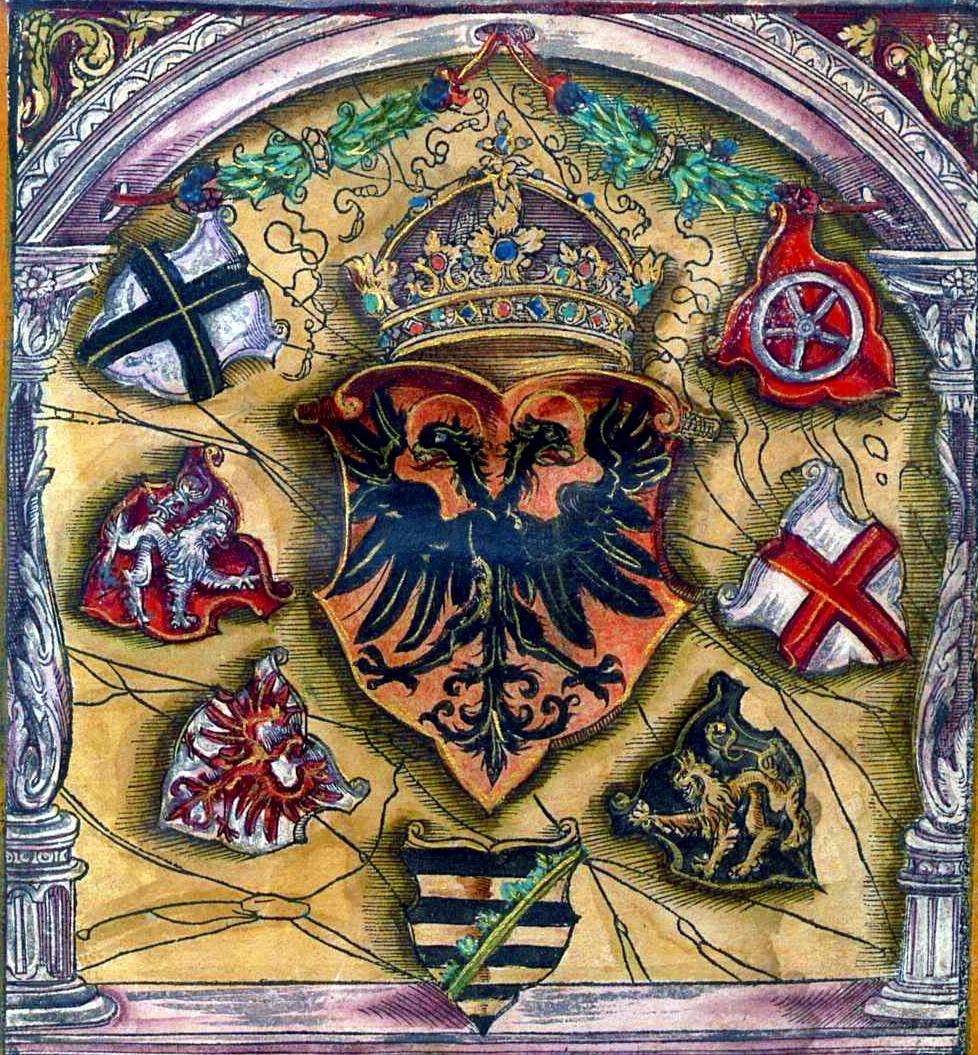
\includegraphics[width = 5cm, height= 7cm]{Kaiserwappen.jpg}
\caption{Wappen des Heiligen Römischen Reiches Deutscher Nation mit den Wappen der Kurfürsten. Fahnenbuch des Jacob Köbel (1545)}
\end{figure}
Der Zusatz „Deutscher Nation“ taucht in der Literatur erstmals 1438 auf, im Antrittsjahr von Albrecht II. 1486 wurde er erstmals in einem Gesetzestext erwähnt. Die Betonung des deutschen Charakters des Römischen Reiches verstärkte sich seit Ende des 15. Jahrhunderts, als die Macht des Kaisers in Reichsitalien de facto nicht mehr ins Gewicht fiel und sich im Wesentlichen auf das deutsche Herrschaftsgebiet beschränkte. Auch im Abwehrkampf gegen Karl den Kühnen von Burgund wurde diese Terminologie verwendet.


\section{Neue Legitimation}

Im Reich setzte sich mehr und mehr die Ansicht durch, dass der König (bzw. zukünftige Kaiser) von den Kurfürsten gewählt würde, der dann entweder vom Papst zum Kaiser gekrönt wurde oder – ab der Frühen Neuzeit – ohne Bestätigung durch den Papst in das Kaiseramt nachrückte. Das Papsttum hingegen hatte im Mittelalter immer darauf bestanden, dass es über die „Eignung“ des Kaisers selbst entscheiden könnte – was im Reich auf erheblichen Widerstand stieß (siehe Staufer). Der offizielle Königstitel bis zur Ottonenzeit lautete Rex Francorum („König der Franken“) im Regnum Francorum orientalium („Königreich der östlichen Franken“), danach Rex Romanorum („Römischer König“).

Nach der Kaiserkrönung wurde die Titulatur um den Zusatz semper Augustus ergänzt, der aber teilweise auch schon vor der Kaiserkrönung gebraucht wurde. Dieser Titel wurde als „allzeit Mehrer des Reiches“ verdeutscht, da man Augustus fälschlich vom lateinischen Verb augere („vermehren, vergrößern“) ableitete. Der Begriff Mehrer stand dabei für die Pflicht des Herrschers, die Rechte des Imperiums zu schützen und zu erhalten. Konkret bedeutete dies, dass der Kaiser die Entfremdung von Reichsrechten wie Regalien (wie in Italien) oder den Verlust von Gebieten (wie im westlichen Grenzraum an Frankreich) zu verhindern hatte.
\cite{Kintzinger}


  %!TEX root = thesis.tex

\chapter{Neuzeit}
\label{chapter-evaluation}

Seit der Annahme des Titels Erwählter Römischer Kaiser durch Maximilian I. (1508) wurde dieser von allen nachfolgenden römisch-deutschen Königen beim Antritt der Alleinherrschaft und der offiziellen Krönung verwendet, etwa durch Karl V. 1520. Auf eine Krönung durch den Papst wurde fortan verzichtet, mit Ausnahme Karls V., der sich 1530 nachträglich durch den Papst in Bologna krönen ließ.

Der letzte Kaiser des Heiligen Römischen Reiches Deutscher Nation, Franz II. führte als Titel \textit{divina favente clementia electus Romanorum Imperator, semper Augustus} („von Gottes Gnaden erwählter Römischer Kaiser, zu allen Zeiten Mehrer des Reichs“) und war nur in einem Nebentitel \textit{Germaniae Rex} („König in Germanien“; seit Maximilian I. 1508). Nachdem sich Napoleon Bonaparte selbst zum Kaiser der Franzosen proklamiert hatte, rief sich der Kaiser am 11. August 1804 als Franz I. zum Kaiser von Österreich aus, um einem Statusverlust vorzubeugen und die habsburgische Kaiserkrone weiterzuführen. Durch die Gründung des Rheinbundes unter französischem Protektorat und unter dem Druck eines französischen Ultimatums sah sich Franz II. gezwungen, am 6. August 1806 die römisch-deutsche Kaiserkrone niederzulegen. Aus Sorge, dass die Reichskrone in französische Hände gelangen könnte und die österreichischen Länder durch die lehnsrechtliche Bindung an das Reich de jure unter napoleonische Herrschaft gelangen könnten, löste er das Reich als Ganzes auf, womit er seine Kompetenzen als Reichsoberhaupt überschritt.
\cite{Schubert}


  %!TEX root = thesis.tex

\chapter{Zusammenfassung und Ausblick}
\label{chapter-fazit}

Wie in der Einleitung schon erwähnt befasst sich die Arbeit auf den Werdegang durch die verschiedenen Zeitalter, es wurde auf das Früh- und Hochmittelalter, Spätmittelalter und Neuzeit eingegangen. Diese Zeitalter wurden anhand ihrer Historischen Einzelheiten erklärt. Dadurch ist es dem Leser möglich, das Römische-deutsche Kaiserreich zu verstehen und nachzuvollziehen, was innerhalb dieser Zeitalter geschieht.
In diesem Artikel wurde nicht auf die einzelnen Kaiser eingegangen und deren Erfolge bzw. Niederlagen. Ein weiteres Aufgabengebiet wäre somit, die einzelnen Kaiser zu analysieren und deren Informationen die für das Thema relevant sind aufzulisten und zusammenhänge zu finden.
\cite{Schulze}
\begin{figure}[H]
\centering

\includegraphics[width = 5cm, height= 5cm]{GrossesWappen.png}
\caption{Großes Wappen des römisch-deutschen Kaisers Joseph II. (1765)}
\end{figure}

  \appendix

  %!TEX root = thesis.tex

\chapter{Anhang}

Dieser Anhang enthält tiefergehende Informationen, die nicht zur eigentlichen Arbeit gehören.

\section{Abschnitt des Anhangs}

In den meisten Fällen wird kein Anhang benötigt, da sich selten Informationen ansammeln, die nicht zum eigentlichen Inhalt der Arbeit gehören. Vollständige Quelltextlisting haben in ausgedruckter Form keinen Wort und gehören daher weder in die Arbeit noch in den Anhang. Darüber hinaus gehören Abbildungen bzw. Diagramme, auf die im Text der Arbeit verwiesen wird, auf keinen Fall in den Anhang.

  \backmatter

  \cleardoublepage
  \phantomsection
  \pdfbookmark{Abbildungsverzeichnis}{listoffigures}
  \listoffigures

  \cleardoublepage
  \phantomsection
  \pdfbookmark{Tabellenverzeichnis}{listoftables}
  \listoftables

  \cleardoublepage
  \phantomsection
  \pdfbookmark{Definitions- und Theoremverzeichnis}{listoftheorems}
  \renewcommand{\listtheoremname}{Definitions- und Theoremverzeichnis}
  \listoftheorems[ignoreall,show={Lemma,Theorem,Korollar,Definition}]

  %!TEX root = thesis.tex

\cleardoublepage
\phantomsection
\pdfbookmark{Abkürzungsverzeichnis}{abbreviations}
\chapter*{Abkürzungsverzeichnis}
\label{section-abbrevs}

\begin{tabularx}{\textwidth}{lX}
  ABA & alternierender Büchi-Automat, engl. \emph{a}lternating \emph{B}üchi \emph{a}utomaton\\
  AFA & alternierender endlicher Automat, engl. \emph{a}lternating \emph{f}inite \emph{a}utomaton\\
  BA & Büchi-Automat, engl. \emph{B}üchi \emph{a}utomaton\\
  BNF & Normalform kontextfreier Grammatiken, engl. \emph{B}ackus--\emph{N}aur \emph{f}orm\\
  DFA & endlicher Automat, engl. \emph{d}eterministic \emph{f}inite \emph{a}utomaton
\end{tabularx}


  \cleardoublepage
  \phantomsection
  \pdfbookmark{Literaturverzeichnis}{bibliography}
  \bibliography{literature}
\end{document}
